\chapter{系统实现}

\setlength{\textfloatsep}{10pt plus 2pt minus 2pt}
\setlength{\floatsep}{10pt plus 2pt minus 2pt}
\setlength{\intextsep}{10pt plus 2pt minus 2pt}
\setlength{\abovecaptionskip}{4pt}
\setlength{\belowcaptionskip}{0pt}
\renewcommand{\topfraction}{0.9}
\renewcommand{\bottomfraction}{0.8}
\renewcommand{\textfraction}{0.08}
\renewcommand{\floatpagefraction}{0.8}

本章结合前端项目 \texttt{front}、后端项目 \texttt{back} 以及当前可运行环境，对系统实现过程进行说明。内容围绕开发环境、核心功能、实现难点和界面展示展开，重点说明各项设计如何在代码层落地，并给出关键流程图、代码片段和界面截图。

\section{开发环境搭建}

\subsection{硬件与基础软件配置}
系统采用前后端分离方式实现。后端基于 Spring Boot 构建 REST 接口和流式生成服务，前端基于 Vue 3 构建交互界面与在线预览模块，数据持久化由 MySQL 完成。开发与调试过程主要在 Windows 11 环境下进行。为了保证前端构建、后端编译和数据库服务可以并行运行，本地环境需要具备稳定的多任务处理能力。运行环境中的 Java 17、Spring Boot、Vue 3 与 Vite 版本选择均与官方长期支持或当前稳定文档保持一致（Java SE 17 Documentation）（Spring Boot Reference Documentation）（Vue.js Documentation）（Vite Documentation）\cite{oraclejava17docs2025}\cite{springbootdocs2025}\cite{vuedocs2025}\cite{vitedocs2025}。

本次开发环境的硬件与操作系统配置见表 \ref{tab:chapter5-hardware}。其中处理器与操作系统版本来源于本地命令行环境的实际检测结果，内存容量在论文中按可稳定运行本项目的建议配置给出。该配置能够满足前端热更新、后端单元测试、MySQL 服务和论文编译同时运行的要求。

\begin{table}[!htbp]
\centering
\caption{开发环境硬件与操作系统配置}
\label{tab:chapter5-hardware}
\small
\begin{tabular}{@{}p{0.22\textwidth}p{0.28\textwidth}p{0.34\textwidth}@{}}
\toprule
项目 & 本次环境配置 & 说明 \\
\midrule
处理器 & Intel64 Family 6 Model 154，20 个逻辑处理器 & 满足前后端并行构建与本地数据库服务运行需求 \\
体系结构 & AMD64 & 与 Java 17、Node.js 20 和 MySQL 8 的运行环境兼容 \\
操作系统 & Windows 11 64 位 & 作为论文编写、代码开发和本地部署统一环境 \\
内存 & 16 GB 及以上（建议） & 保证 Vite、Spring Boot、MySQL 与 XeLaTeX 同时运行时仍有足够余量 \\
\bottomrule
\end{tabular}
\end{table}

软件环境配置见表 \ref{tab:chapter5-software}。版本信息来自项目依赖文件和本地运行结果。后端采用 Spring Boot 3.4.3，前端主要依赖 Vue 3、Vite、Pinia、Vue Router 与 Element Plus。数据库驱动使用 \texttt{mysql-connector-j}，构建工具分别为 Maven 与 npm。

\begin{table}[!htbp]
\centering
\caption{开发环境软件配置清单}
\label{tab:chapter5-software}
\small
\begin{tabular}{@{}p{0.18\textwidth}p{0.20\textwidth}p{0.18\textwidth}p{0.30\textwidth}@{}}
\toprule
类别 & 软件或框架 & 版本 & 用途 \\
\midrule
JDK & OpenJDK & 17.0.12 & 运行 Spring Boot 后端服务 \\
后端框架 & Spring Boot & 3.4.3 & 提供控制器、服务层、数据访问与任务调度能力 \\
构建工具 & Apache Maven & 3.9.9 & 后端依赖管理、编译与测试执行 \\
数据库 & MySQL & 8.4.0 & 保存用户、项目、任务、版本和审计数据 \\
前端运行时 & Node.js & 20.15.1 & 运行 Vite 开发服务器与前端构建脚本 \\
前端包管理 & npm & 10.7.0 & 管理前端依赖与执行构建命令 \\
前端框架 & Vue & 3.5.29 & 构建单页应用与响应式界面 \\
前端构建工具 & Vite & 6.4.1 & 提供本地开发服务器与生产构建能力 \\
状态管理 & Pinia & 3.0.4 & 管理认证、项目、工作区和草稿状态 \\
路由管理 & Vue Router & 4.6.4 & 管理登录、生成页、历史页和管理页的页面跳转 \\
界面组件库 & Element Plus & 2.13.5 & 提供表单、表格、分页、标签与消息提示组件 \\
\bottomrule
\end{tabular}
\end{table}

\subsection{项目依赖安装与启动方式}
后端配置文件中定义了服务端口、数据库连接、模型调用地址、会话有效期和成本控制参数。实际部署时，数据库账号、数据库口令和模型密钥应通过配置文件或部署环境注入，不应在前端代码中暴露。当前项目使用 \texttt{spring.jpa.hibernate.ddl-auto=update} 自动维护表结构，适合论文原型系统的开发阶段，但在正式生产环境中仍应结合显式迁移脚本控制变更过程。

为了验证环境可用性，本研究分别执行了依赖检查、单元测试和前端构建。后端 \texttt{mvn test} 通过，前端 \texttt{npm test} 与 \texttt{npm run build} 通过，说明解析器、安全扫描器、前端预览逻辑与打包流程可以正常工作。JUnit 5 与 Vitest 分别对应后端和前端的主流单元测试工具链，能够满足当前原型系统对断言、测试组织和脚本运行的需要（JUnit 5 User Guide）（Vitest Guide）\cite{junit5docs2025}\cite{vitestdocs2025}。主要启动与验证命令见表 \ref{tab:chapter5-verify}。

\begin{table}[!htbp]
\centering
\caption{项目启动与验证命令}
\label{tab:chapter5-verify}
\small
\begin{tabular}{@{}p{0.20\textwidth}p{0.34\textwidth}p{0.30\textwidth}@{}}
\toprule
操作对象 & 主要命令 & 结果说明 \\
\midrule
后端版本检查 & \texttt{java -version}，\texttt{mvn -version} & 确认 JDK 17 与 Maven 3.9.9 可用 \\
后端测试 & \texttt{mvn test} & 解析器与安全扫描器相关测试通过 \\
前端版本检查 & \texttt{node -v}，\texttt{npm -v} & 确认 Node.js 20.15.1 与 npm 10.7.0 可用 \\
前端测试 & \texttt{npm test} & 前端工具函数与预览逻辑测试通过 \\
前端构建 & \texttt{npm run build} & 生成生产构建产物，说明路由与页面组件可正常打包 \\
数据库检查 & \texttt{mysql --version} & 确认 MySQL 8.4.0 服务端工具可用 \\
\bottomrule
\end{tabular}
\end{table}

在实际启动顺序上，系统通常先启动 MySQL 数据库，再启动后端服务，最后启动前端开发服务器。登录成功后，前端会通过项目状态存储创建默认项目并同步工作区标识，之后生成页、历史页和管理页即可共享同一组认证信息与项目上下文。该启动方式与项目当前代码中的 \texttt{useAuthStore}、\texttt{useProjectStore}、\texttt{useWorkspaceStore} 的初始化顺序保持一致，有助于减少页面首次进入时的上下文缺失问题。

\section{核心功能实现}

\subsection{生成任务创建与流式回传实现}
系统最核心的功能是根据用户输入的需求描述生成 Vue 单文件组件。该过程由后端任务创建接口与流式接口协同完成。当前实现中，\texttt{GenerationController} 提供 \texttt{/generations} 与 \texttt{/generations/\{taskId\}/stream} 两个入口。前者用于创建任务记录，后者用于建立 SSE 连接并持续回传生成过程。

\texttt{GenerationService.createTask} 在创建任务时会完成三类校验。其一是读取当前登录用户，确认请求已经通过认证拦截器。其二是校验项目归属与工作区归属，避免用户跨项目访问任务资源。其三是检查提示词与组件名长度，防止过长输入直接进入生成链路。校验通过后，系统创建一条状态为 \texttt{PENDING} 的任务记录，并写入项目、工作区、需求描述、约束 JSON、组件名和模型标识等信息。

\texttt{GenerationStreamService.generateAndStream} 在异步线程池中执行真正的生成链路。该方法先通过 \texttt{runningMap} 为任务建立互斥锁，再更新任务状态为 \texttt{GENERATING}，随后检查用户当日 token 配额，最后决定是命中缓存还是调用模型接口。当前实现还将 token 片段通过 \texttt{emit(..., "token", ...)} 持续发送给浏览器，因此前端可以实时显示模型输出，而不必等待整段代码完全生成后再刷新界面。典型生成流程见图 \ref{fig:chapter5-flow-generation}。

\begin{figure}[!htbp]
\centering
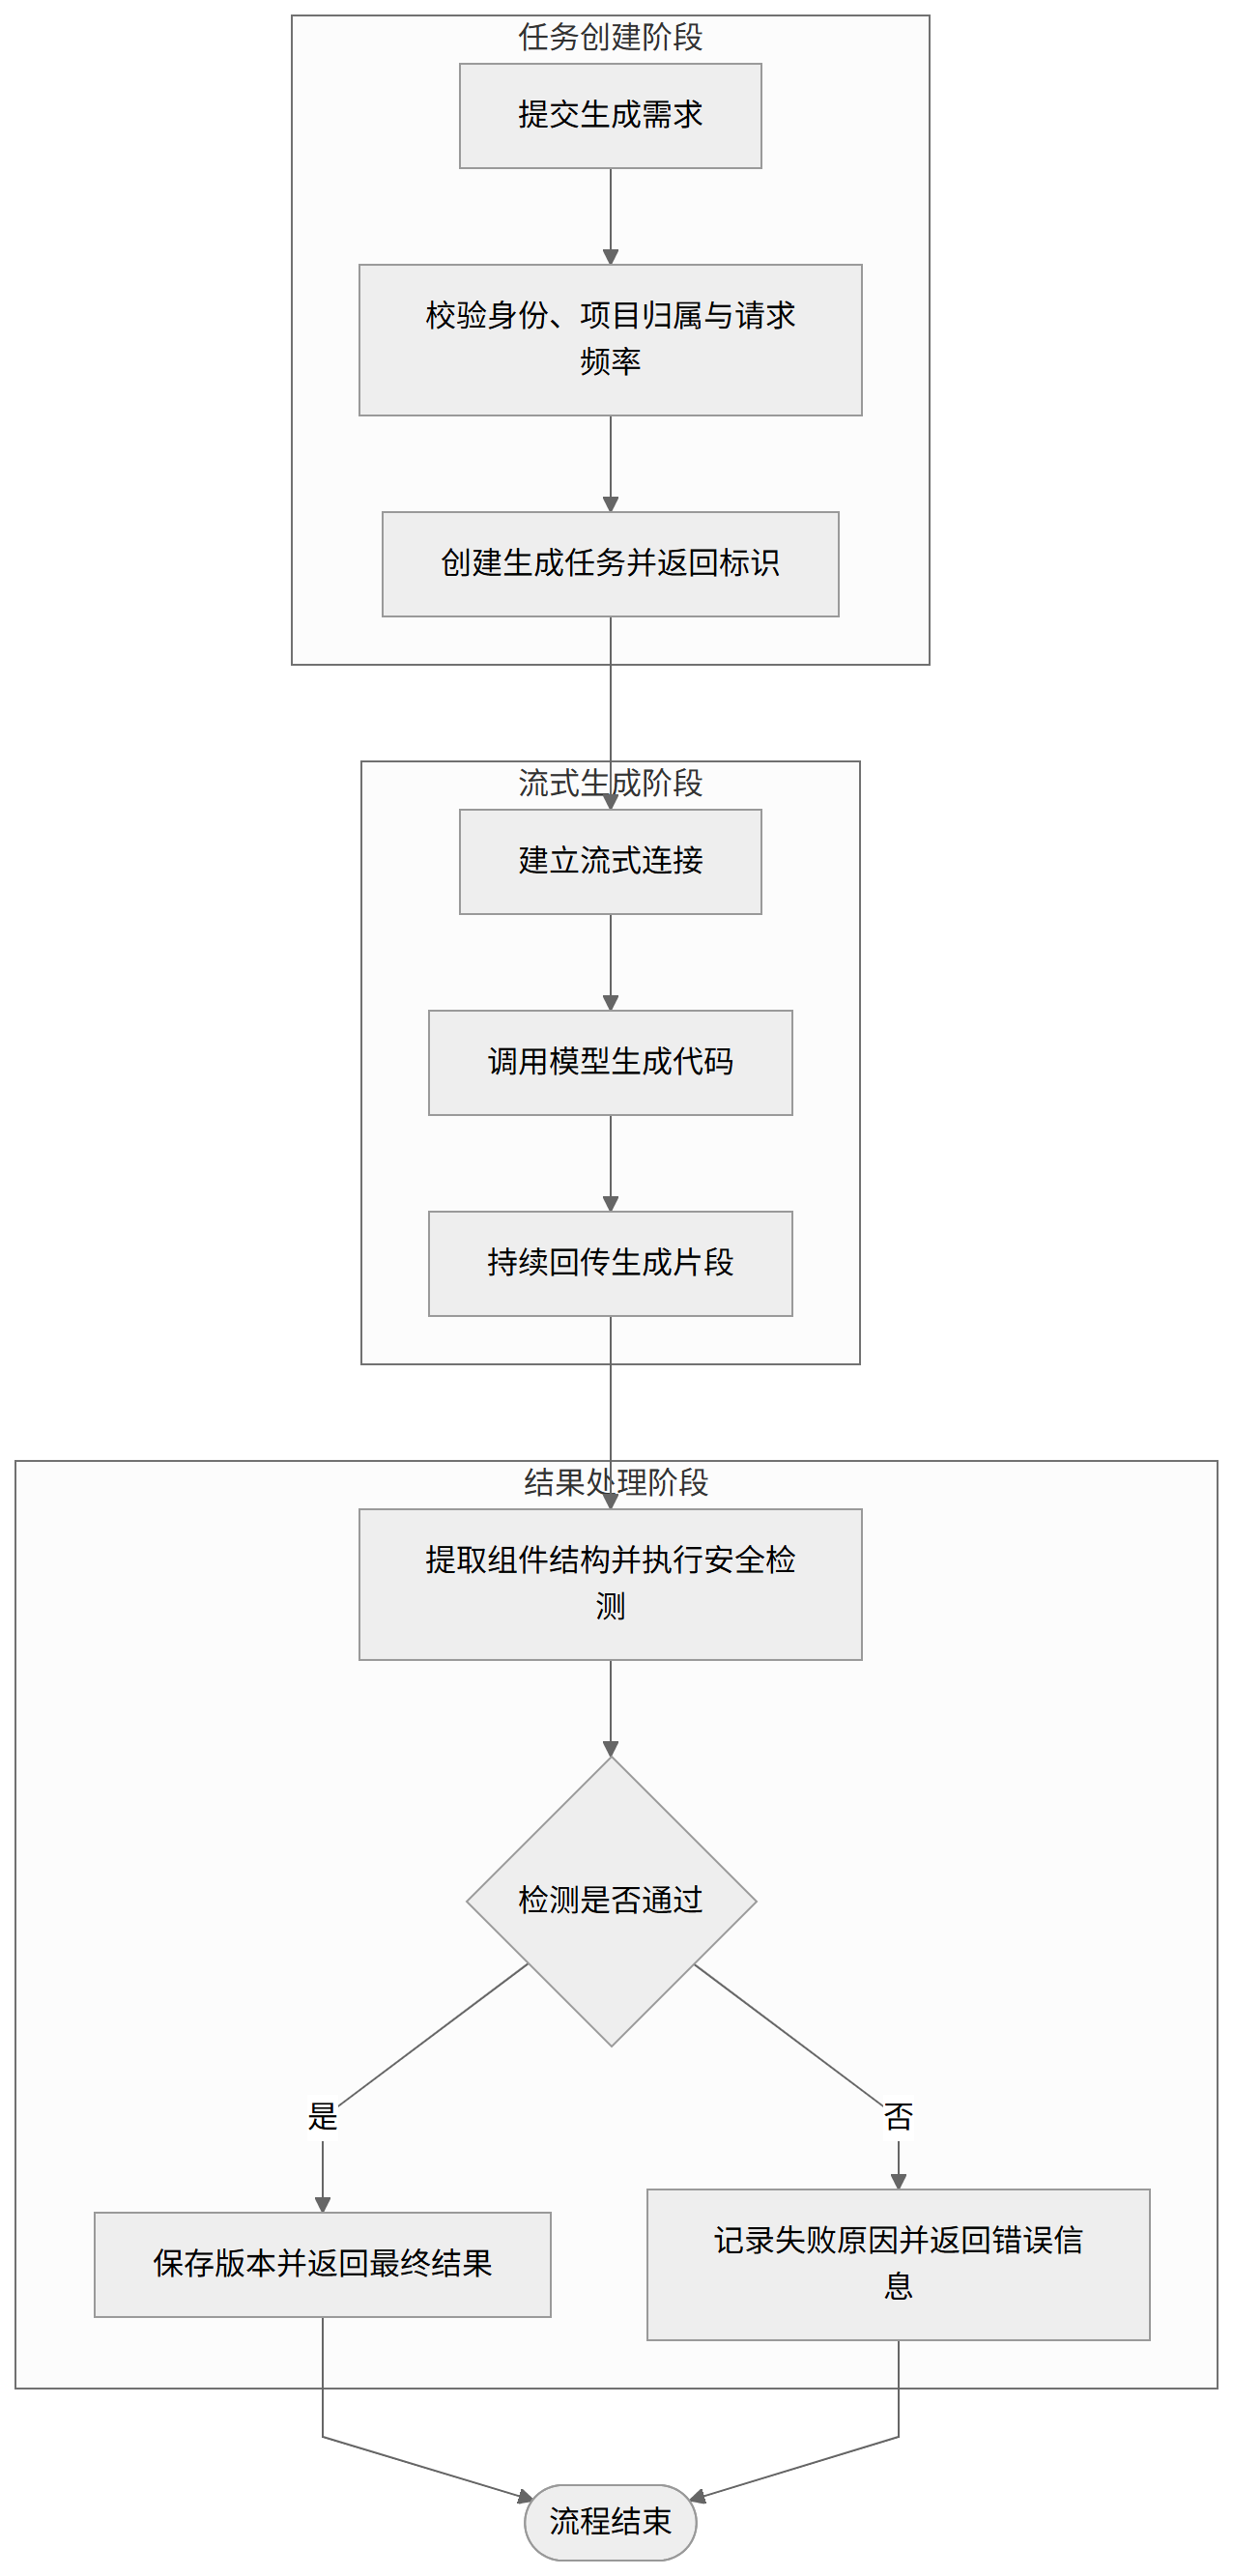
\includegraphics[width=0.96\textwidth,height=0.46\textheight,keepaspectratio]{figures/generation-stream-flow.png}
\caption{组件生成典型实现流程}
\label{fig:chapter5-flow-generation}
\end{figure}

任务互斥逻辑是流式生成稳定运行的基础。系统没有简单依赖数据库字段判断任务是否正在执行，而是先在内存中建立原子锁，再配合任务状态字段完成双重控制。关键代码片段如下：

\begin{quote}
\small
\begin{verbatim}
AtomicBoolean lock =
    runningMap.computeIfAbsent(
        taskId, ignored -> new AtomicBoolean(false));
if (!lock.compareAndSet(false, true)) {
    emitError(emitter, "Task is already generating");
    emitter.complete();
    return;
}
\end{verbatim}
\end{quote}

前端生成页 \texttt{GeneratorView.vue} 对应上述链路。页面在点击“生成”按钮后，先调用 \texttt{createGenerationTask} 创建任务，再调用 \texttt{streamGenerationTask} 发起流式请求。考虑到系统需要携带 \texttt{X-Auth-Token}、\texttt{X-Project-Id} 与 \texttt{X-Workspace-Key} 等自定义请求头，前端没有直接使用原生 \texttt{EventSource}，而是通过 \texttt{fetch + ReadableStream} 手动解析 SSE 数据帧。这样既保留了流式返回特性，也能够与系统现有鉴权方式保持一致。

当前事件处理逻辑按事件类型更新界面状态。收到 \texttt{started} 事件后，页面切换到生成中状态；收到 \texttt{token} 事件后，页面将 token 追加到流式输出区域；收到 \texttt{final\_code} 事件后，页面保存最新版本编号并更新代码编辑区；收到 \texttt{error} 事件后，页面直接显示错误信息。这种设计将任务创建、任务执行和界面刷新拆分为清晰的阶段，便于定位链路中的具体故障点。

\subsection{结构化解析、安全校验与版本落库实现}
大模型返回的内容并不总是严格符合 Vue 单文件组件格式，系统因此在生成完成后增加了解析与校验步骤。后端解析器 \texttt{SfcCodeExtractor} 会先尝试抽取三引号代码块，再分别提取 \texttt{template}、\texttt{script} 和 \texttt{style} 三个区域。若某一部分缺失，则使用默认内容补齐；若脚本标签存在但未声明 \texttt{setup}，则自动转换为 \texttt{<script setup>} 形式。这样可以保证落库结果始终具备统一结构。

解析器的兜底逻辑直接决定了系统面对不完整输出时的可恢复能力。关键片段如下：

\begin{quote}
\small
\begin{verbatim}
String template = extractOrDefault(code, TEMPLATE,
        "<template>\n  <div>Generated component</div>\n</template>");
String script = ensureScriptSetup(
        extractOrDefault(code, SCRIPT, "<script setup>\n</script>"));
String style = extractOrDefault(code, STYLE, "<style scoped>\n</style>");
\end{verbatim}
\end{quote}

在解析结果生成后，系统会调用 \texttt{CodeSafetyScanner} 执行后端安全扫描。当前规则重点覆盖 \texttt{eval}、\texttt{new Function}、远程脚本标签、远程导入、动态 URL 导入、Cookie 访问以及网络请求能力。如果触发阻断规则，任务会被直接标记为失败，系统不会保存组件版本，从而避免高风险代码进入数据库或后续预览环节。该过程使“可运行”与“可保存”之间增加了一层明确的安全边界。

版本落库由 \texttt{saveVersion} 与 \texttt{saveCallLog} 两部分组成。前者负责保存结构化代码、版本号、安全级别、编译完整性标记和创建时间，后者负责记录本次模型调用的请求 token、响应 token、总 token、估算费用和耗时。这样做的结果是，历史页既可以按任务查看各版本代码，也可以通过调用日志统计每日成本和资源消耗。核心功能与实现文件的对应关系见表 \ref{tab:chapter5-core}。

\begin{table}[!htbp]
\centering
\caption{核心功能与主要实现文件}
\label{tab:chapter5-core}
\small
\begin{tabular}{@{}p{0.18\textwidth}p{0.30\textwidth}p{0.36\textwidth}@{}}
\toprule
功能项 & 主要实现文件 & 说明 \\
\midrule
任务创建与任务详情 & \texttt{GenerationController}，\texttt{GenerationService} & 创建任务、校验归属、查询任务详情和任务分页列表 \\
流式生成链路 & \texttt{GenerationStreamService}，\texttt{QwenLlmClient} & 异步执行生成流程、回传 token、控制状态流转 \\
结构化代码抽取 & \texttt{SfcCodeExtractor} & 将模型原始输出规范化为可保存的 Vue 单文件组件结构 \\
安全阻断 & \texttt{CodeSafetyScanner} & 对危险脚本、远程资源和网络访问能力进行规则匹配 \\
成本控制与缓存 & \texttt{CostControlService}，\texttt{GenerationCacheService} & 检查配额、估算费用、缓存相同输入的生成结果 \\
在线预览 & \texttt{PreviewSandbox.vue}，\texttt{utils/sfc.js} & 再次解析代码，补齐运行时状态，并将样式限制在预览宿主节点内 \\
历史查看与下载 & \texttt{HistoryView.vue}，\texttt{generation.js} & 查看任务版本列表、打开历史版本、下载 \texttt{.vue} 文件 \\
\bottomrule
\end{tabular}
\end{table}

\subsection{在线预览与版本下载实现}
预览模块用于在浏览器中直接查看生成组件的运行效果。由于生成结果来自大模型输出，系统不能简单把整段代码直接插入页面执行。当前前端实现先使用 \texttt{detectUnsafeCode} 做一次预检查，再通过 \texttt{parseSfcSections} 拆分模板、脚本和样式，随后根据模板中出现的变量、事件与列表来源自动补齐兜底状态，最后再构造临时运行时组件并渲染到预览面板。预览处理流程见图 \ref{fig:chapter5-flow-preview}。

\begin{figure}[!htbp]
\centering
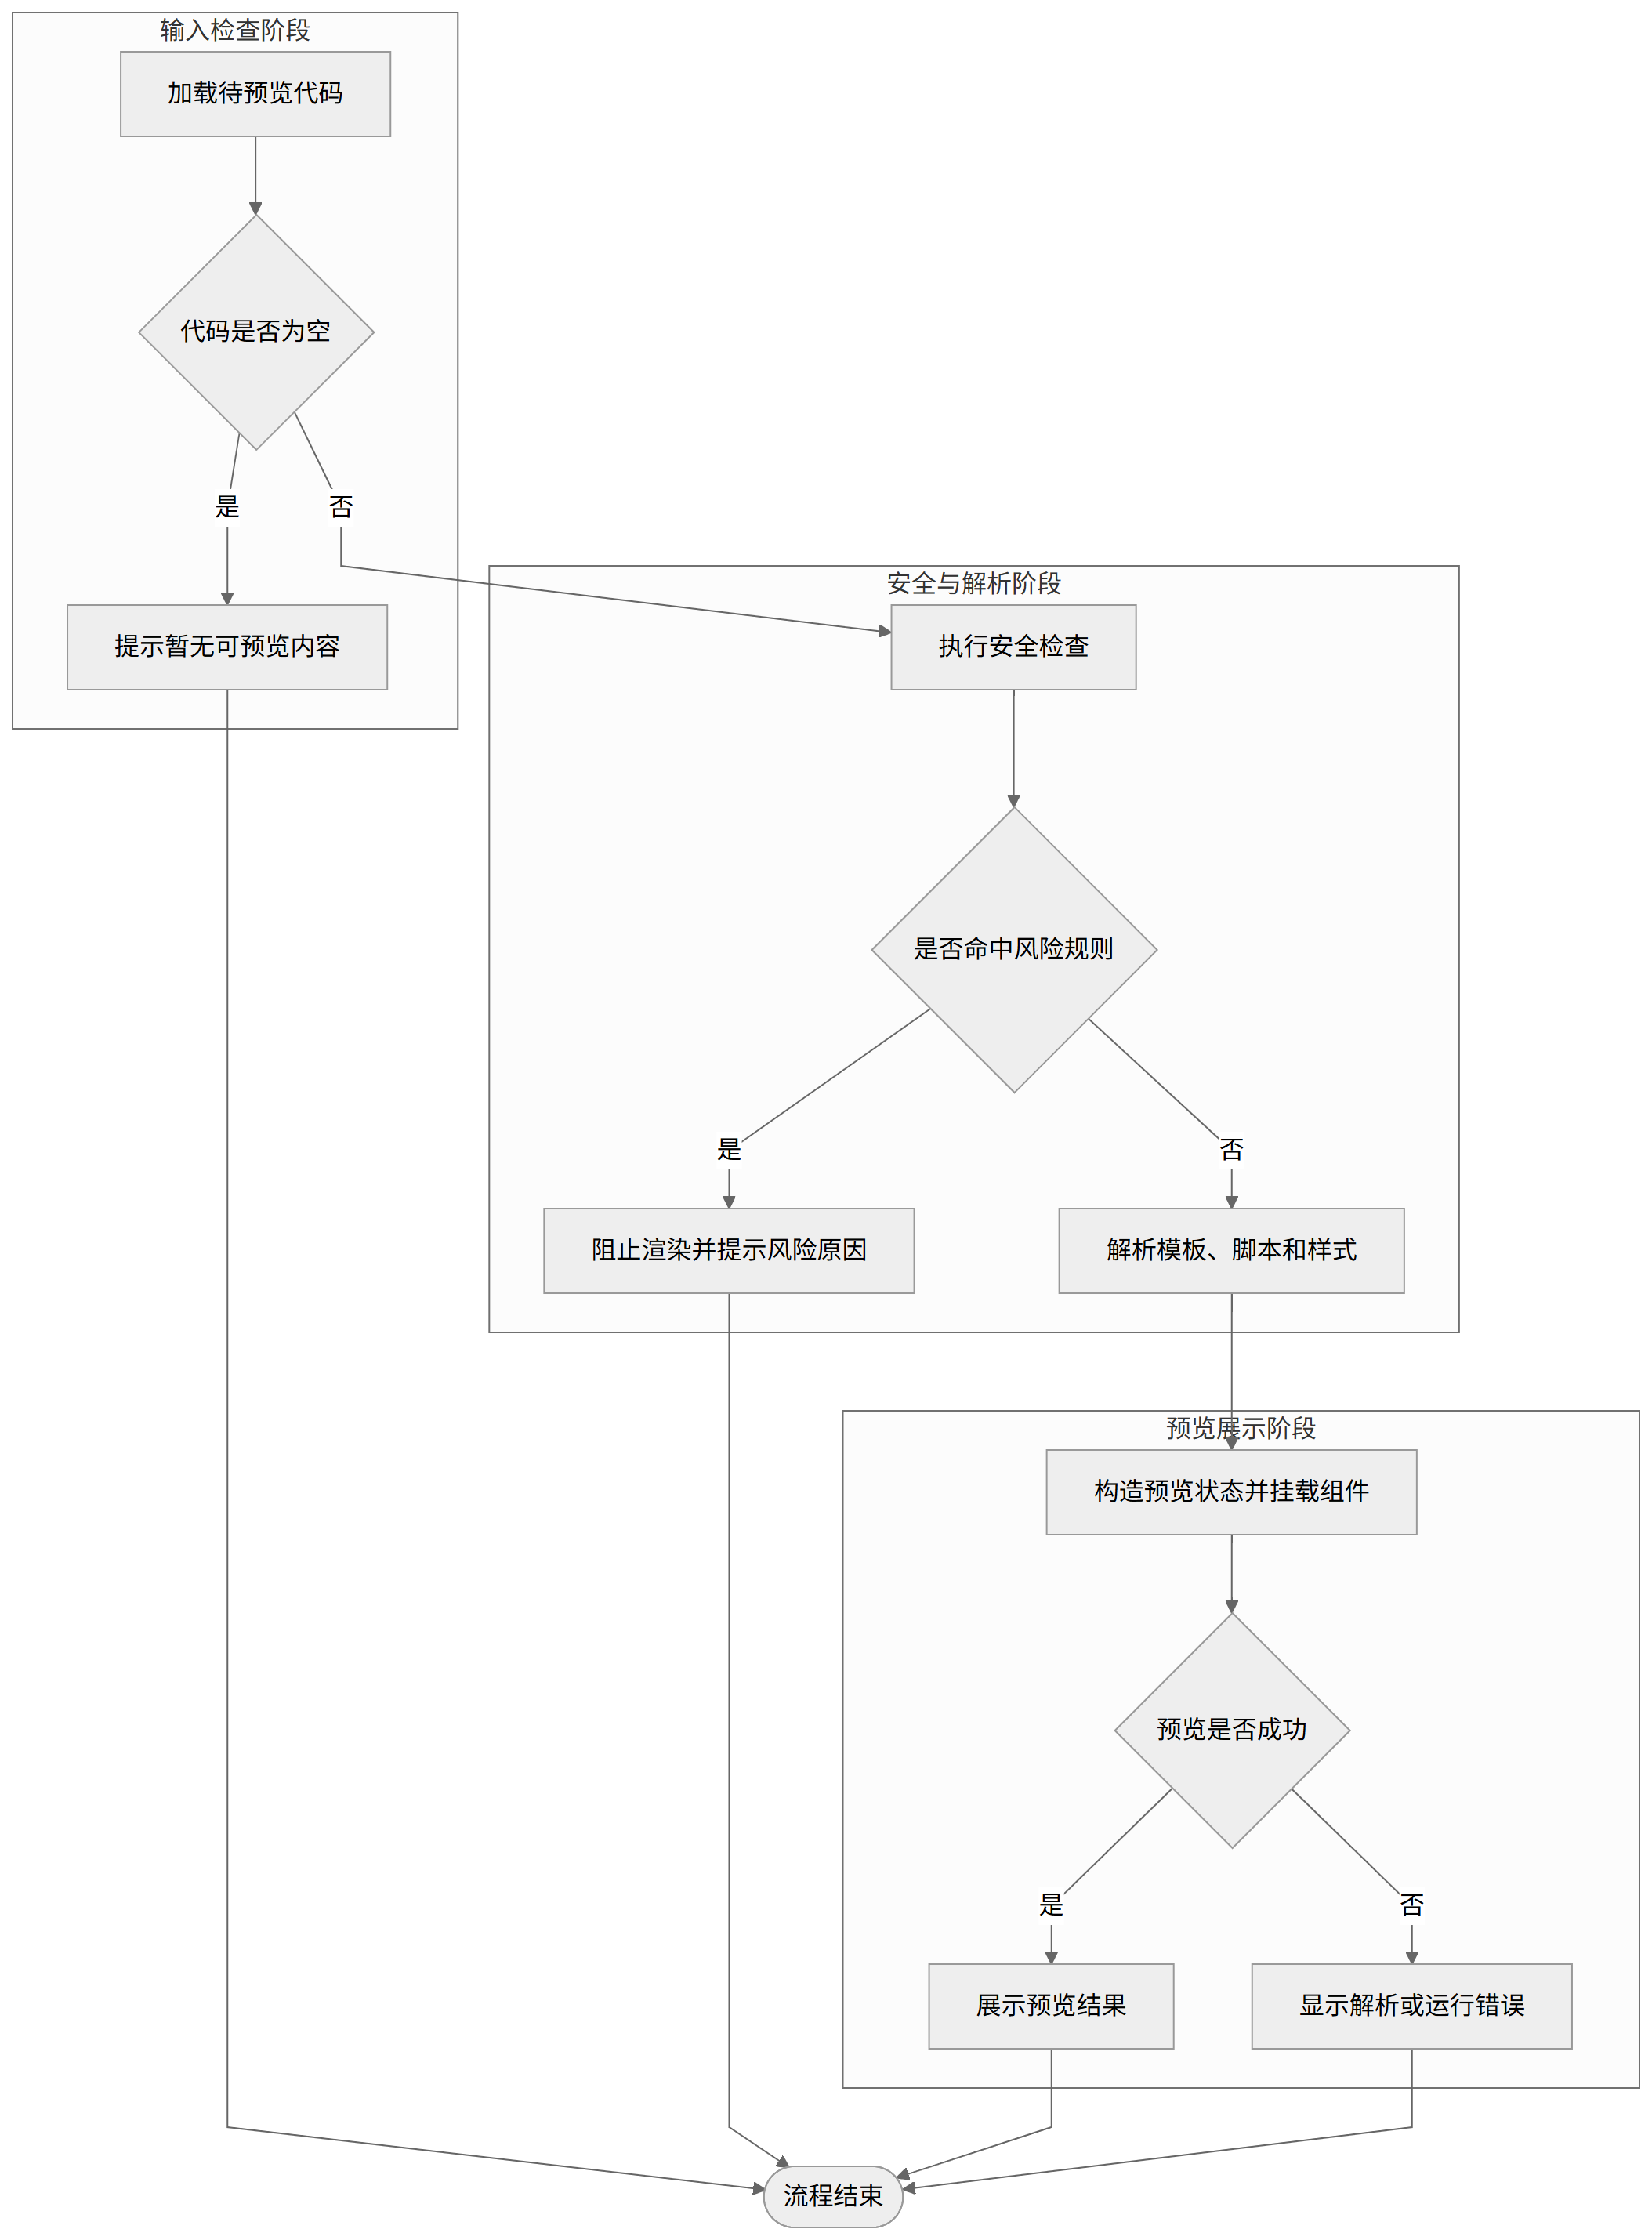
\includegraphics[width=0.96\textwidth,height=0.45\textheight,keepaspectratio]{figures/preview-safety-flow.png}
\caption{在线预览与安全处理流程}
\label{fig:chapter5-flow-preview}
\end{figure}

预览实现的关键不是“把代码跑起来”，而是“只在受控范围内把代码跑起来”。\texttt{PreviewSandbox.vue} 会对生成的样式执行作用域改写，将 \texttt{body}、\texttt{html}、\texttt{:root} 等选择器统一替换为 \texttt{.preview-host}，从而避免预览代码污染整个页面。相关处理片段如下：

\begin{quote}
\small
\begin{verbatim}
if (selector === "body" || selector === "html" || selector === ":root") {
    return hostSelector;
}
if (selector.startsWith(hostSelector)) {
    return selector;
}
return `${hostSelector} ${selector}`;
\end{verbatim}
\end{quote}

为了提高预览成功率，系统还实现了模板变量推断与默认值补齐机制。当前逻辑会从 \texttt{v-model}、\texttt{v-for}、插值表达式和事件绑定中抽取变量名，再根据变量名称和上下文特征推断默认类型，例如将 \texttt{users}、\texttt{items} 推断为数组，将 \texttt{total}、\texttt{count} 推断为数值，将 \texttt{visible}、\texttt{enabled} 推断为布尔值。这一机制虽然不替代真实业务数据，但足以支撑组件结构和交互雏形的展示。

版本下载实现较为直接。当前历史页和生成页都会调用 \texttt{downloadVersion} 接口获取 Blob 数据，再由浏览器创建临时下载链接并触发保存。后端保存的内容本身已经是规范化后的 Vue 单文件组件文本，因此下载结果可以直接作为 \texttt{.vue} 文件复用。该方式保持了预览代码、数据库版本内容与下载文件内容的一致性，避免出现“页面显示内容”和“实际导出文件”不一致的问题。

\section{难点解决方案}

\subsection{大模型输出不稳定的兼容处理}
系统实现中最明显的难点是大模型输出并不稳定。同一类需求在不同时间可能返回完整组件，也可能只返回模板片段、缺少脚本标签，或者将说明文字和代码混合在一起。如果直接把原始输出作为版本结果保存，后续预览、下载和历史复用都会受到影响。

为了解决这一问题，后端在模型调用完成后立即执行结构化抽取。系统先从原始结果中提取代码块，再按标签划分三个区域；若脚本与样式不完整，则自动补齐默认内容；若脚本不是 \texttt{setup} 格式，则转换为 \texttt{script setup}。这一策略将“输出是否完美”转换为“输出是否能够被修复并继续进入下一个环节”，从而显著提升了版本保存成功率。

\subsection{流式任务并发与状态一致性处理}
另一个难点是流式任务存在较长执行时间，用户可能重复点击“生成”或“重新生成”按钮。如果系统仅依赖前端按钮禁用，很容易在网络抖动、页面刷新或重复请求条件下出现同一任务并发执行的问题。当前实现采用了“前端状态控制 + 后端任务状态 + 服务内原子锁”三层约束方式。前端在请求发出后立即将 \texttt{loading} 状态置为真，后端在流式入口处判断任务当前状态，同时通过 \texttt{runningMap} 保证同一任务只能有一个活跃执行链路。

在任务结果管理方面，系统将任务状态划分为 \texttt{PENDING}、\texttt{GENERATING}、\texttt{SUCCEEDED} 和 \texttt{FAILED}。状态变化由服务层方法集中维护。任务开始执行时调用 \texttt{markTaskGenerating}，执行成功时调用 \texttt{markTaskSucceeded}，执行失败时调用 \texttt{markTaskFailed}。这样做有两个直接效果：任务列表页可以准确显示当前状态，异常发生时也能在数据库中保留错误信息和完成时间，便于排查问题。对于重复输入的生成请求，系统还引入缓存服务，将模型名、组件名、提示词、约束与演示数据开关组合为哈希键，从而减少重复生成造成的额外成本。

\subsection{预览隔离与风险阻断方案}
在线预览模块涉及代码执行，因此实现难点不仅在于正确渲染，还在于避免危险代码影响宿主页面。当前系统采用前后端双层控制。后端阻止高风险代码入库，前端在加载版本代码后再次执行风险检测，并将样式作用域限制在预览容器内部。这样即使后端规则未来扩展不完整，前端仍然具备额外的保护层。

系统对主要难点的优化前后处理方式见表 \ref{tab:chapter5-compare}。表中可以看到，当前方案并未试图通过单一规则解决全部问题，而是将结构化处理、状态控制、缓存和安全校验分别放在合适的执行节点上。这样既降低了链路耦合度，也使每个故障点都具有可观测的状态输出。

\begin{table}[!htbp]
\centering
\caption{主要实现难点的优化前后对比}
\label{tab:chapter5-compare}
\footnotesize
\begin{tabular}{@{}p{0.17\textwidth}p{0.24\textwidth}p{0.24\textwidth}p{0.23\textwidth}@{}}
\toprule
问题场景 & 优化前表现 & 优化后方案 & 改进效果 \\
\midrule
模型输出结构不完整 & 模板、脚本或样式缺失时无法保存，历史页和下载页缺少可用版本 & 使用 \texttt{SfcCodeExtractor} 抽取代码块并补齐默认模板、脚本与样式 & 生成结果具有统一结构，后续预览与下载链路可以继续执行 \\
同一任务重复触发 & 网络重试或重复点击会导致同一任务并发执行，状态覆盖风险较高 & 使用前端 \texttt{loading} 控制、后端状态流转和 \texttt{runningMap} 原子锁联合约束 & 降低重复执行概率，任务状态和版本号更稳定 \\
重复请求成本过高 & 相同提示词每次都重新调用模型，增加耗时与 token 消耗 & 使用 \texttt{GenerationCacheService} 对相同输入进行哈希缓存 & 缩短二次请求响应时间，减少重复调用成本 \\
预览代码污染宿主页面 & 组件样式可能直接影响导航栏、表单或全局字体 & 使用 \texttt{scopeCssToHost} 将样式限制在 \texttt{.preview-host} 容器中 & 预览结果与宿主页面隔离，页面样式更稳定 \\
高风险脚本进入预览 & 恶意代码可能通过远程导入、网络请求等方式扩大影响范围 & 后端 \texttt{CodeSafetyScanner} 与前端 \texttt{detectUnsafeCode} 双层拦截 & 预览执行边界更清晰，高风险代码不会进入运行阶段 \\
\bottomrule
\end{tabular}
\end{table}

\section{系统界面展示}
系统界面围绕“登录进入项目、生成组件、查看历史版本、管理员治理”四类主要操作展开。生成页承担系统最核心的工作流，因此采用单页集中布局，将输入区、流式输出区、代码区和预览区放在同一界面内，减少用户在多个页面间来回切换。生成页界面截图见图 \ref{fig:chapter5-ui-generator}。

\begin{figure}[!htbp]
\centering
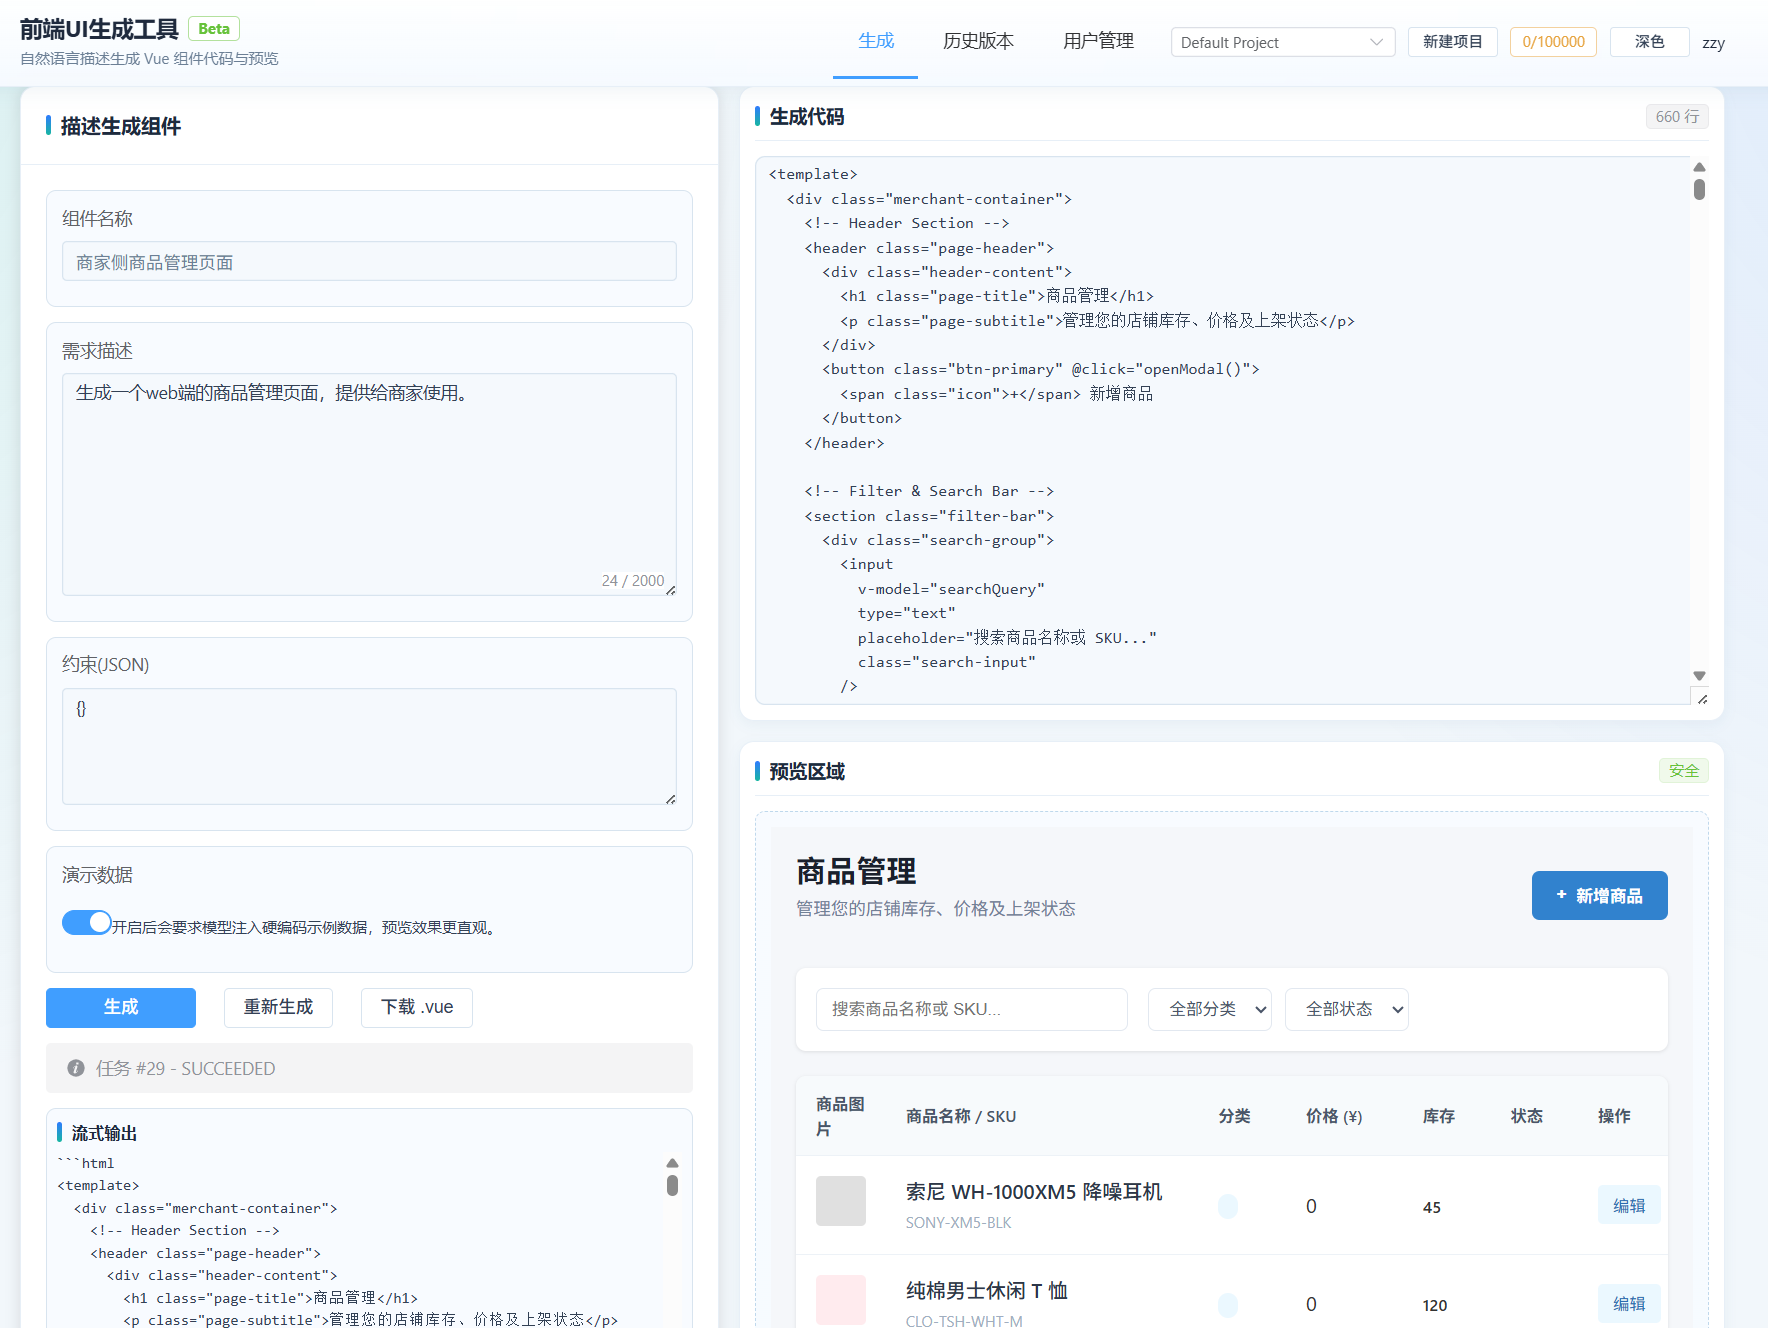
\includegraphics[width=0.96\textwidth,height=0.48\textheight,keepaspectratio]{figures/主界面.png}
\caption{生成页面界面截图}
\label{fig:chapter5-ui-generator}
\end{figure}

从图 \ref{fig:chapter5-ui-generator} 可以看出，页面左侧集中布置组件名称、需求描述、约束 JSON、演示数据开关以及生成、重新生成、下载等操作按钮；页面右侧上半部分显示代码编辑区，下半部分显示在线预览区。流式输出区域位于表单下方，用于实时展示大模型返回过程。该布局与 \texttt{GeneratorView.vue} 中的双列栅格结构一致，适合持续观察生成状态并快速调整提示词。

除生成页外，系统还提供登录注册页、历史页和管理员页面，用于支撑完整业务流程。登录注册页负责建立会话身份；历史页用于查看任务列表和版本列表，并支持打开历史版本与下载组件文件；管理员页面用于查询用户、调整角色和启停账号。登录注册页界面截图见图 \ref{fig:chapter5-ui-login}，历史页与用户管理页界面截图分别见图 \ref{fig:chapter5-ui-history} 和图 \ref{fig:chapter5-ui-user-admin}。

\begin{figure}[!htbp]
\centering
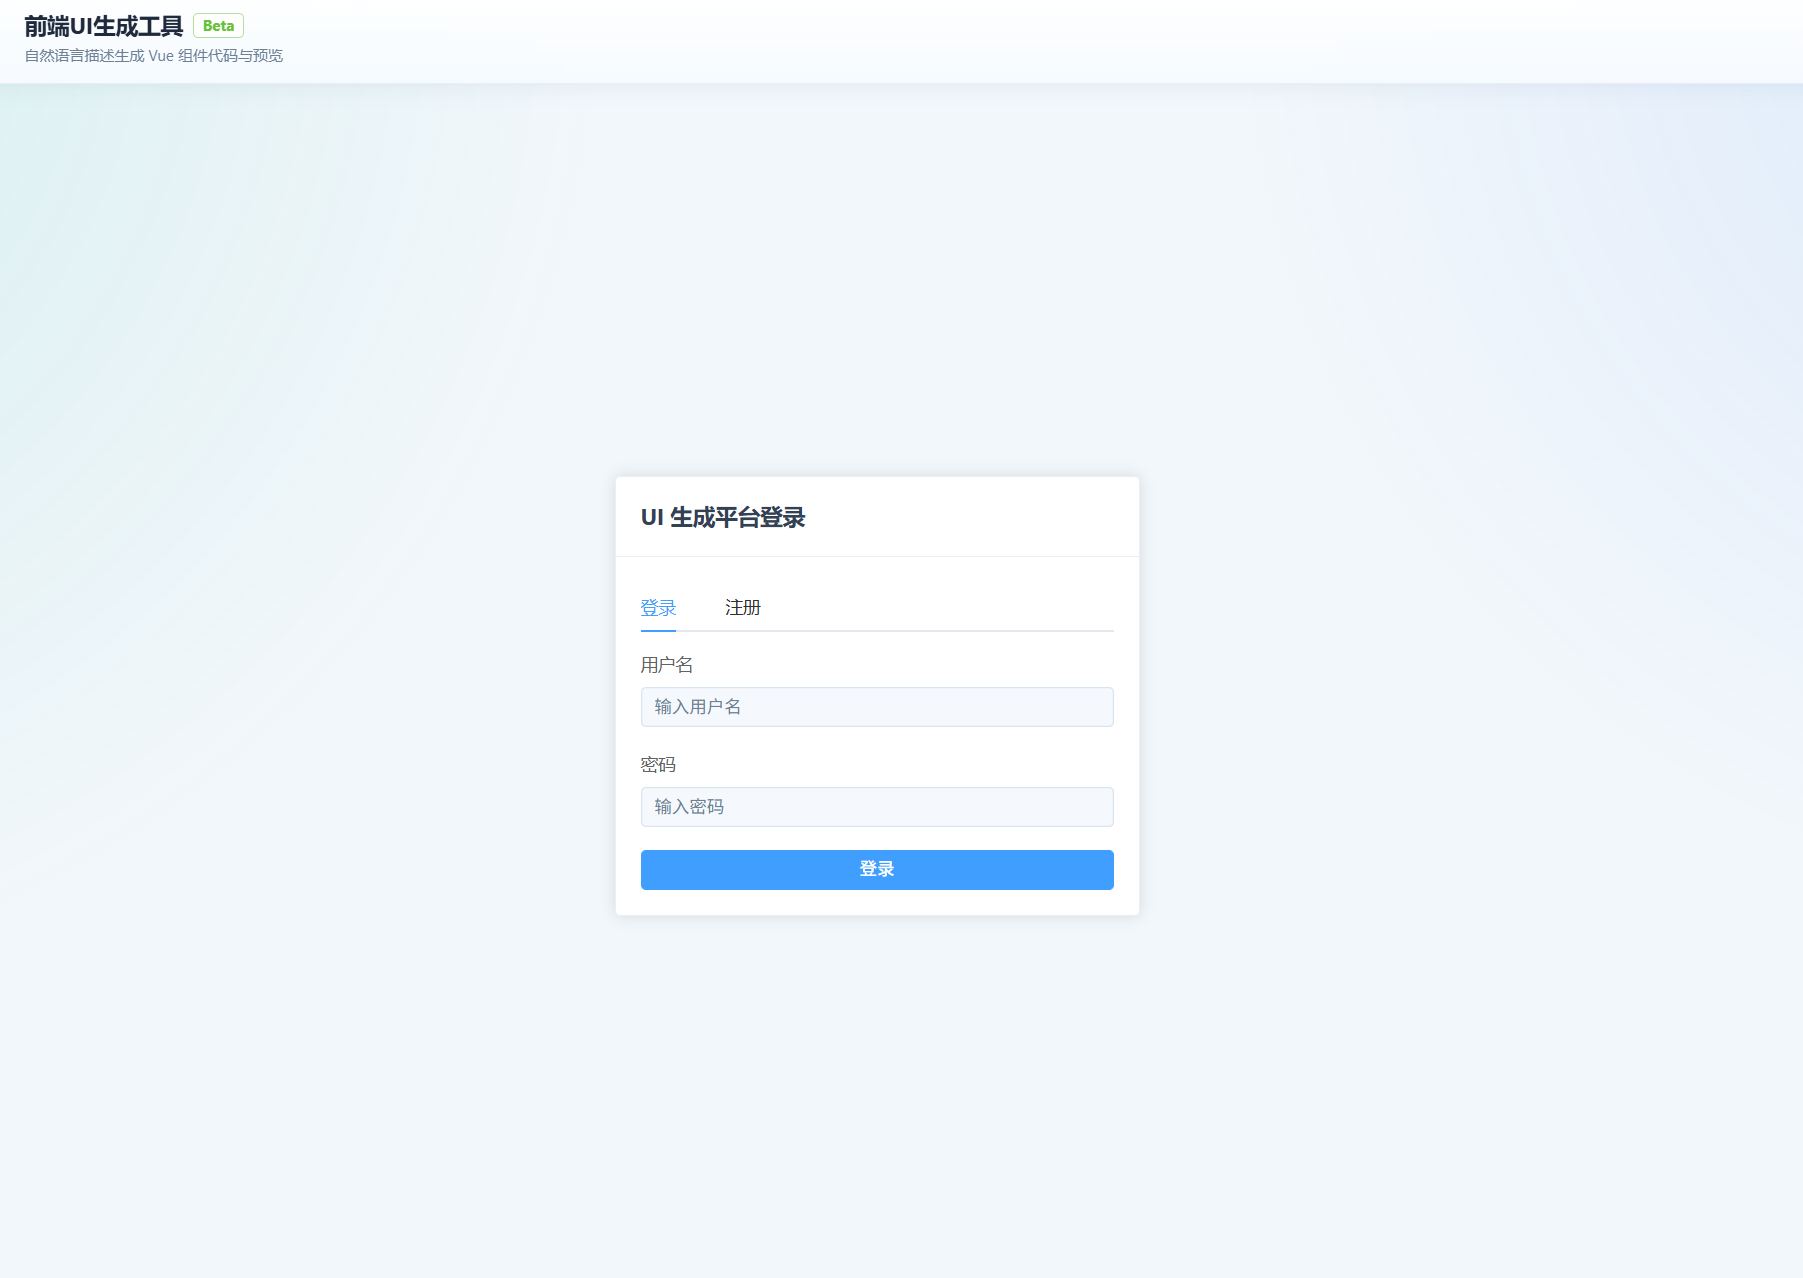
\includegraphics[width=0.72\textwidth,height=0.34\textheight,keepaspectratio]{figures/登录注册.png}
\caption{登录注册页面界面截图}
\label{fig:chapter5-ui-login}
\end{figure}

\begin{figure}[!htbp]
\centering
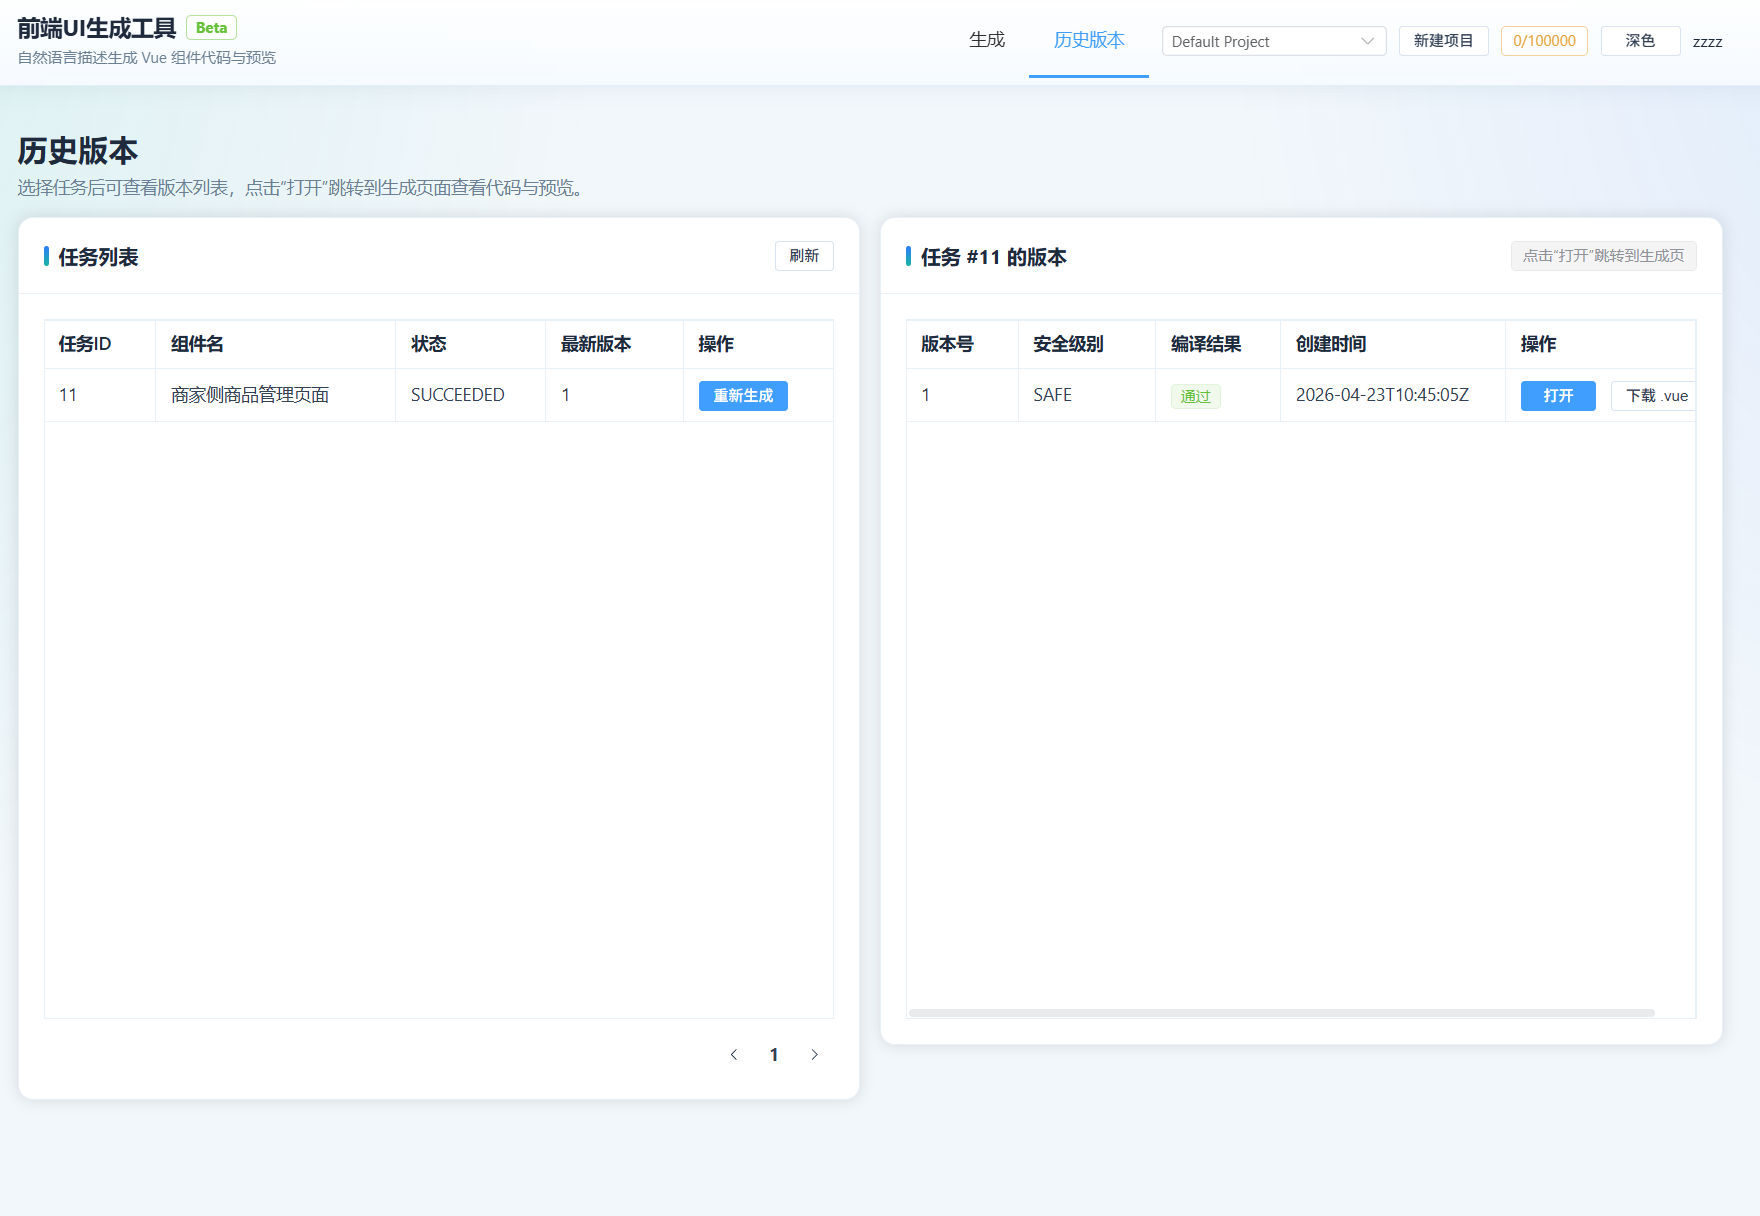
\includegraphics[width=0.96\textwidth,height=0.40\textheight,keepaspectratio]{figures/版本管理.png}
\caption{历史版本页面界面截图}
\label{fig:chapter5-ui-history}
\end{figure}

\begin{figure}[!htbp]
\centering
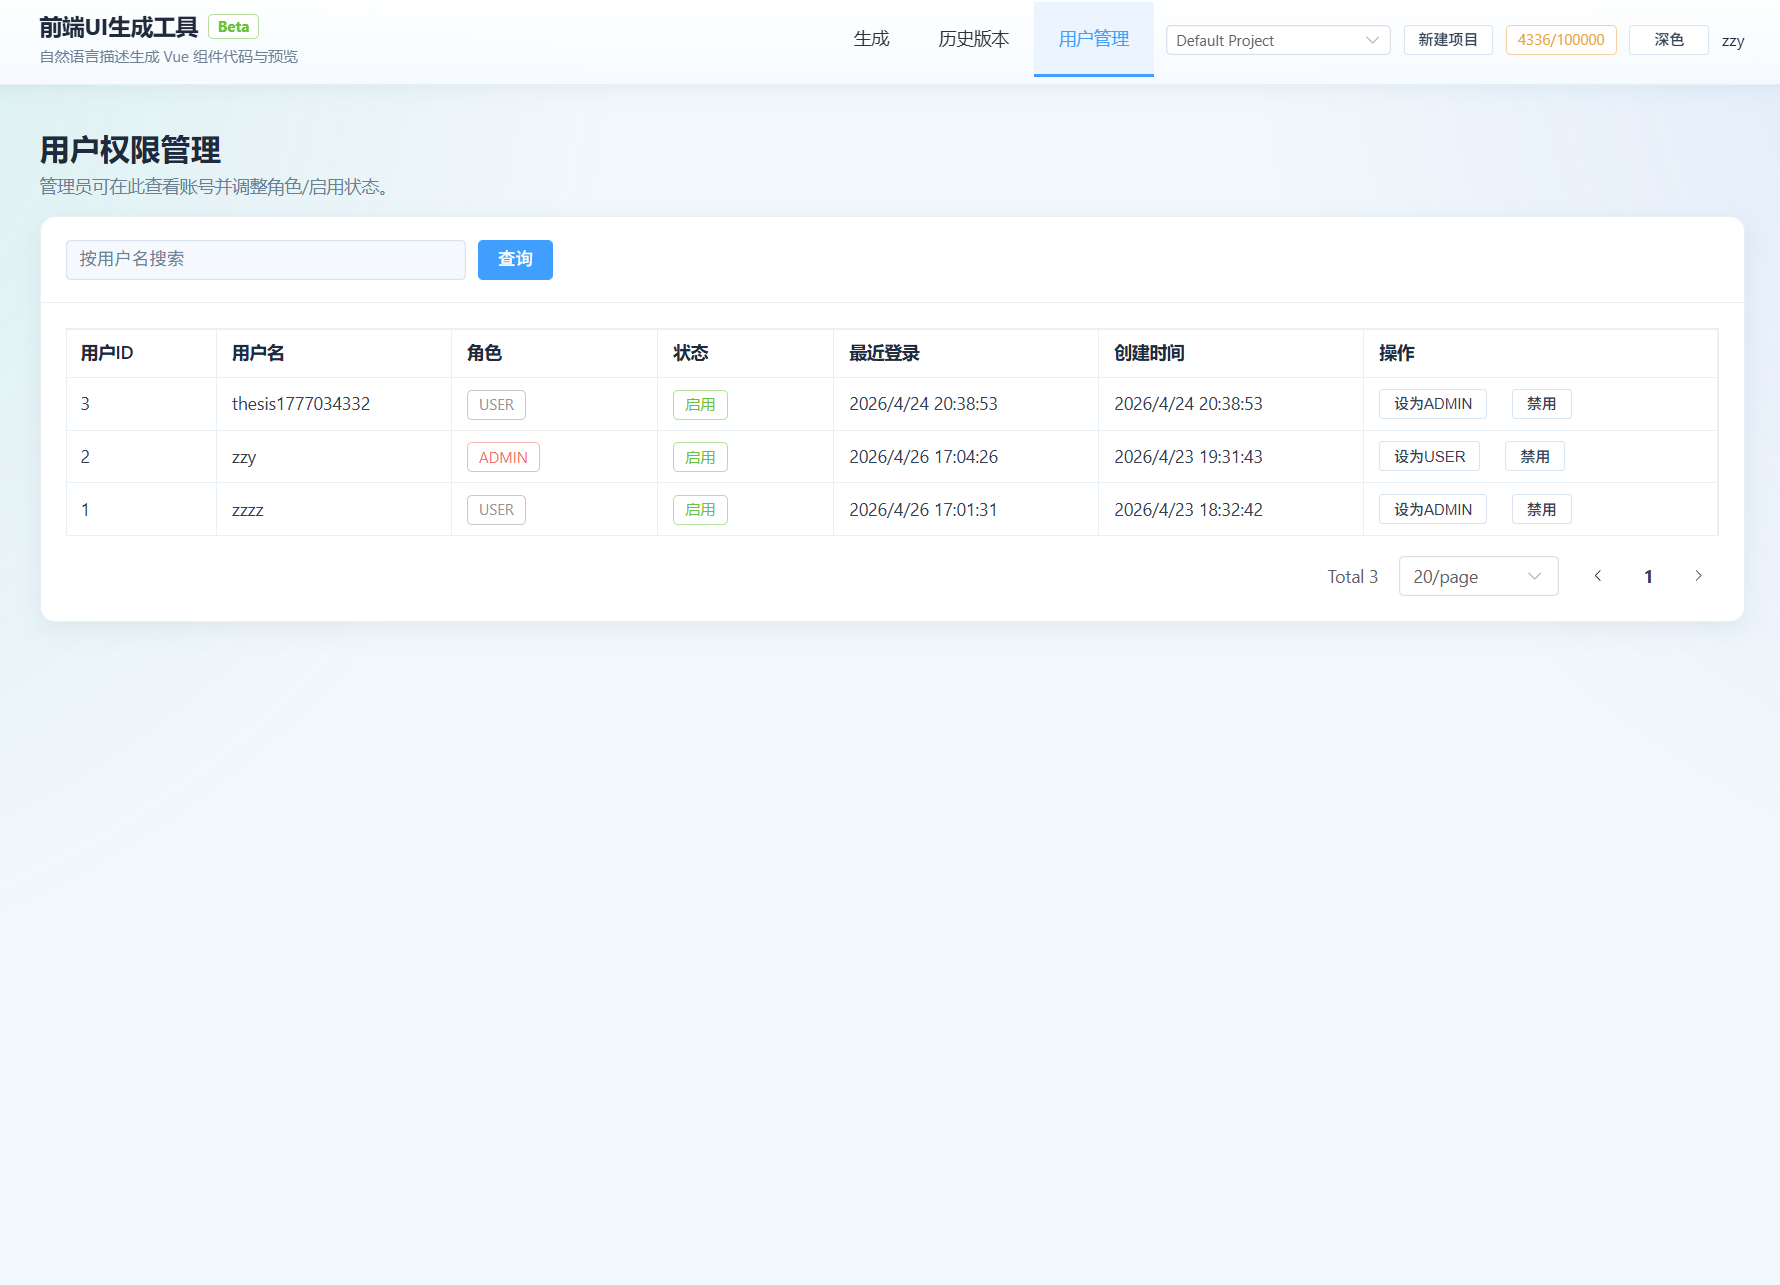
\includegraphics[width=0.96\textwidth,height=0.40\textheight,keepaspectratio]{figures/用户管理.png}
\caption{用户管理页面界面截图}
\label{fig:chapter5-ui-user-admin}
\end{figure}

登录注册页保持单卡片结构，注册与登录入口集中在同一页面中，有利于减少首次使用步骤，并让访客用户更快进入系统。历史页采用左右并列布局，左侧为任务分页列表，右侧为所选任务对应的版本列表，适合在保留任务上下文的情况下查看多个历史版本。用户管理页采用搜索栏、表格与操作按钮组合方式，便于完成用户筛选、角色切换和账号状态维护。整体界面实现与前端路由划分、状态存储和后端接口设计保持一致，说明系统设计已经在界面层完成了可操作的工程落地。
